% Glossareinträge
\newacronym{cpu}{CPU}{Central Processing Unit}
% Ende Glossareinträge

\chapter{Hardware}

Die Hardware besteht aus einem Raspberry Pi, \todo{genauere Beschreibung}
\section{Der Raspberry Pi}
\begin{wrapfigure}{r}{0.5\textwidth}
 \vspace{-16pt}
 \centering 
 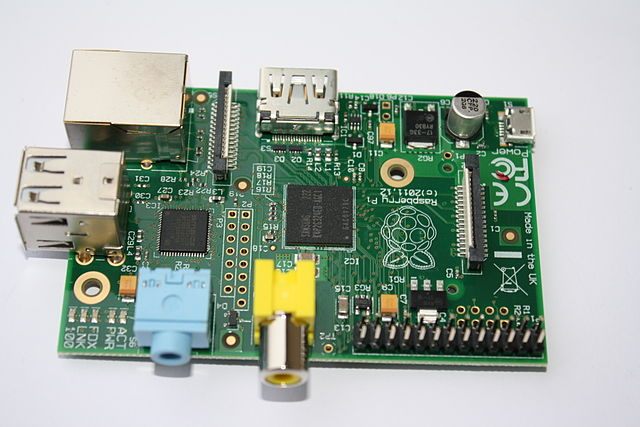
\includegraphics[width=0.45\textwidth]{figures/raspberry.jpg}
 \caption[Raspberry Pi - Modell B]{Raspberry Pi - Modell B\footnotemark}
 \vspace{-50pt}
\end{wrapfigure}
\footnotetext{\cite{rasp_bild}}
Der \textit{Rasperry Pi} ist ein Einplatinencomputer, der 2012 von der  \textit{Raspberry Pi Foundation} auf den Markt gebracht wurde. 
\subsection{Geschichte}
Ursprünglich war er als günstiger Computer gedacht, um britischen Jugendlichen das Programmieren näher zu bringen. An der \textit{University of Cambridge} stellte man fest, dass die Vorkenntnisse von Studienanfängern immer geringer wurden, weil sie -- sowohl privat als auch in der Schule -- sich immer weniger mit der Funktionsweise von Computern und Programmen beschäftigen. Daher wollte man einen Computer entwickeln, mit dem die Jugendlichen experimentieren können.
\footcite{aboutraspberry}$^,$\todo{absolut geschummelt}
\footcite{wiki:raspi_geschichte}

\subsection{Technische Daten}
Die Technik in einem Raspberry Pi ist vergleichbar mit der eines Smartphones. Der Raspberry Pi hat eine \acrshort{cpu} mit 700 MHz, welche auf bis zu 1 GHz übertaktbar ist und je nach Modell 256 oder 512 MB Arbeitspeicher. Das Betriebsystem (verschiedene Linux-Distributionen stehen zur Auswahl